\documentclass{my-article}
\usepackage{my-coverpage}
\usepackage{my-codespace}

\usepackage[utf8]{inputenc}
\usepackage[T5]{fontenc}
\usepackage[vietnamese]{babel}

\usepackage{textcomp}
% =========================
% Cover page information
% =========================

\NameUpperUniname{Vietnam National University Ho Chi Minh City}
\NameUniname{Ho Chi Minh City University of Technology}
\NameDeptname{Faculty of Electrical and Electronics Engineering}
\NamePathlogo{./my-chapters/my-images/01_logobachkhoatoi.png}
\NameClass{Digital System Design \\ &  and Verification (EE3213)}
\NameGroup{04}
\NameLesson[\Large]{HOMEWORK REPORT}
\NameTitle[\Huge]{Chương 3 - Thiết kế mạch tổ hợp}
\NameAdvisor{Nguyễn Trung Hiếu}
\NamePlace{Ho Chi Minh}
\NameTime{../../20..}
\NamePathBackground[width=\paperwidth,height=\paperheight]{./my-chapters/my-images/bia.jpg} 
\MemberTableData{
1 & 2213874 & Nguyễn Thanh Tùng & L01 \\ \hline
2 & 2210780 & Nguyễn Đại Đồng & L01 \\ \hline
3 & 2213496 & Nguyễn Quốc Tín & L01 \\ \hline
}

% =========================
% Configuration
% =========================
%--- Header and footer
\fancyhf{}
\fancyhead[L]{\leftmark}
% =========================
% Document
% =========================

\newcommand{\question}[1]{%
	\section*{#1}%
	\addcontentsline{toc}{section}{#1}%
}
\newcommand{\answer}[2]{%
	\subsection*{\textbf{#1}\kern0.2em)~#2}%
	\addcontentsline{toc}{subsection}{#1)}%
}

\newcommand{\finalresult}[1]{%
	\begin{tikzpicture}[baseline=(content.base)]
		\node[draw=red, thick, rounded corners=3pt, inner sep=6pt] (content)
		{\ensuremath{#1}};
	\end{tikzpicture}%
}

\begin{document}
\pagestyle{empty}
\MycoverFinalProject % Cover page
\newpage
\pagestyle{fancy}
\fancyhf{}
\MycountPages{roman}
\renewcommand{\arraystretch}{1.5} % tăng khoảng cách dòng (row height)
\setlength{\parindent}{1cm}
\onehalfspacing
\setlength{\parskip}{6pt} 
\tableofcontents
\listoffigures
\listoftables
\listoflistings
\newpage
\MycountPages{number}
\fancyhead[R]{GVHD: Nguyễn Trung Hiếu}
\fancyfoot[L]{
\includegraphics[width=.02\linewidth]{./my-chapters/my-images/logo_DEE.png}\text{ Department of Electronics}}

%\question{Câu 2}

Thiết kế mạch tổ hợp tìm vị trí bit 1 đầu tiên (tính từ MSB) của chuỗi 24-bit. Cho các standard cell như sau: cổng not, các cổng logic 2 ngõ vào, mux 2-1, mux 4-1.

\answer{a}{Thiết kế mạch chỉ được dùng các standard cell trên.}

Đầu tiên nhóm em sẽ thiết kế từ một bộ tìm kiếm vị trí bit 1 đầu tiên (tính từ MSB) cho một chuỗi 4-bit trước. 

\begin{table}[H]
	\centering
	\begin{tabular}{|c|c|c|c|c|c|c|}
		\hline
		\multicolumn{4}{|c|}{Input} & \multicolumn{2}{c|}{Output} & Zero Flag \\
		\hline
		$X_{3}$ & $X_{2}$ & $X_{1}$ & $X_{0}$ & $Y_{1}$ & $Y_{0}$ & $V$ \\
		\hline
		0 & 0 & 0 & 0 & 0 & 0 & 1 \\
		\hline
		0 & 0 & 0 & 1 & 0 & 0 & 0 \\
		\hline
		0 & 0 & 1 & X & 0 & 1 & 0 \\
		\hline
		0 & 1 & X & X & 1 & 0 & 0 \\
		\hline
		1 & X & X & X & 1 & 1 & 0 \\
		\hline
	\end{tabular}
	\caption{Bảng sự thật của bộ phát hiện bit 1 (Leading one position) cho 4 bit.}
	\label{tab:leading-one-4bit}
\end{table}

Từ bảng \ref{tab:leading-one-4bit}, ta rút gọn và có được mạch như sau:

\begin{figure}[H]
	\centering
	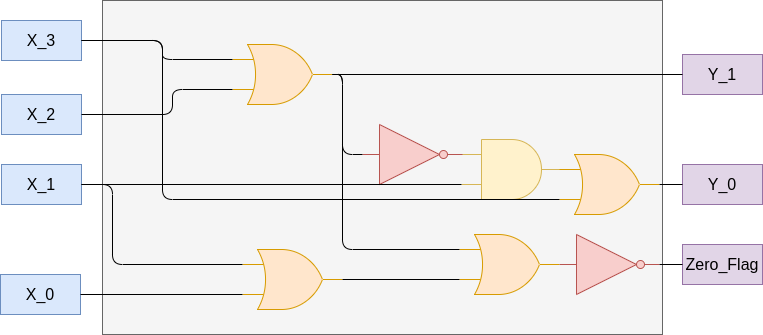
\includegraphics[width=.8\linewidth]{/home/noname/Documents/project_tiny/Ex3/20_doc/my-chapters/my-diagrams/Question2/spec.png}
	\caption{Sơ đồ logic của bộ LOPD 4bit.}
\end{figure}

Từ bộ LOPD 4-bit trên, ta triển khai bộ LOPD 8-bit và bộ LOPD 16-bit như sau:

\begin{figure}[H]
	\centering
	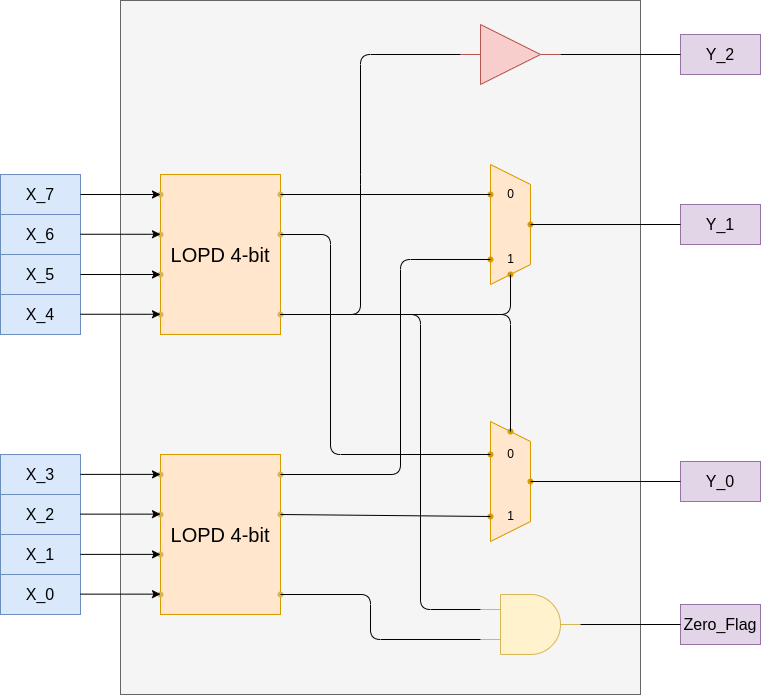
\includegraphics[width=.8\linewidth]{/home/noname/Documents/project_tiny/Ex3/20_doc/my-chapters/my-diagrams/Question2/LOPD_8bit.png}
	\caption{Sơ đồ logic của bộ LOPD 8bit.}
\end{figure}

\begin{figure}[H]
	\centering
	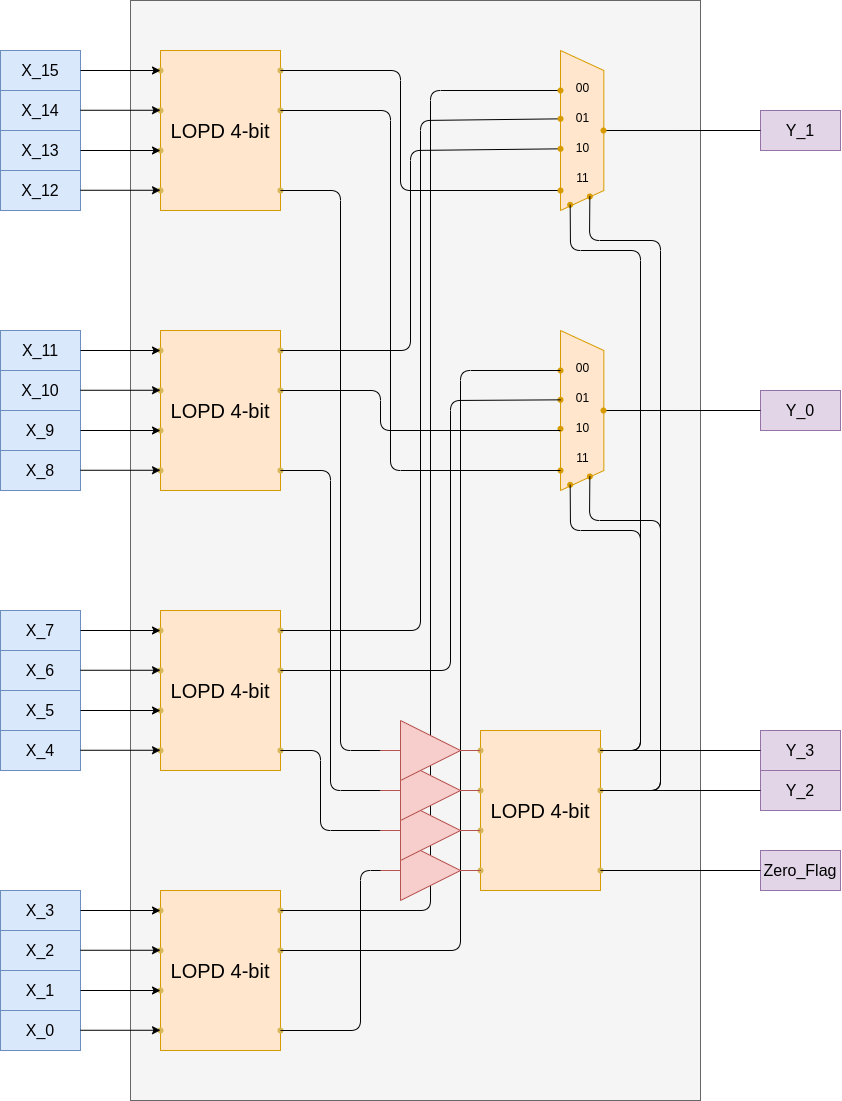
\includegraphics[width=.8\linewidth]{/home/noname/Documents/project_tiny/Ex3/20_doc/my-chapters/my-diagrams/Question2/LOPD_16bit.png}
	\caption{Sơ đồ logic của bộ LOPD 16bit.}
\end{figure}

Từ bộ LOPD 8-bit và LOPD 16-bit trên, ta ghép lại thành 24-bit với LOPD 8-bit vào vị trí 8-bit cao (từ $ 23 \rightarrow 16 $) và bộ LOPD 16-bit vào 16-bit thấp (từ $ 15 \rightarrow 0 $).

\begin{figure}[H]
	\centering
	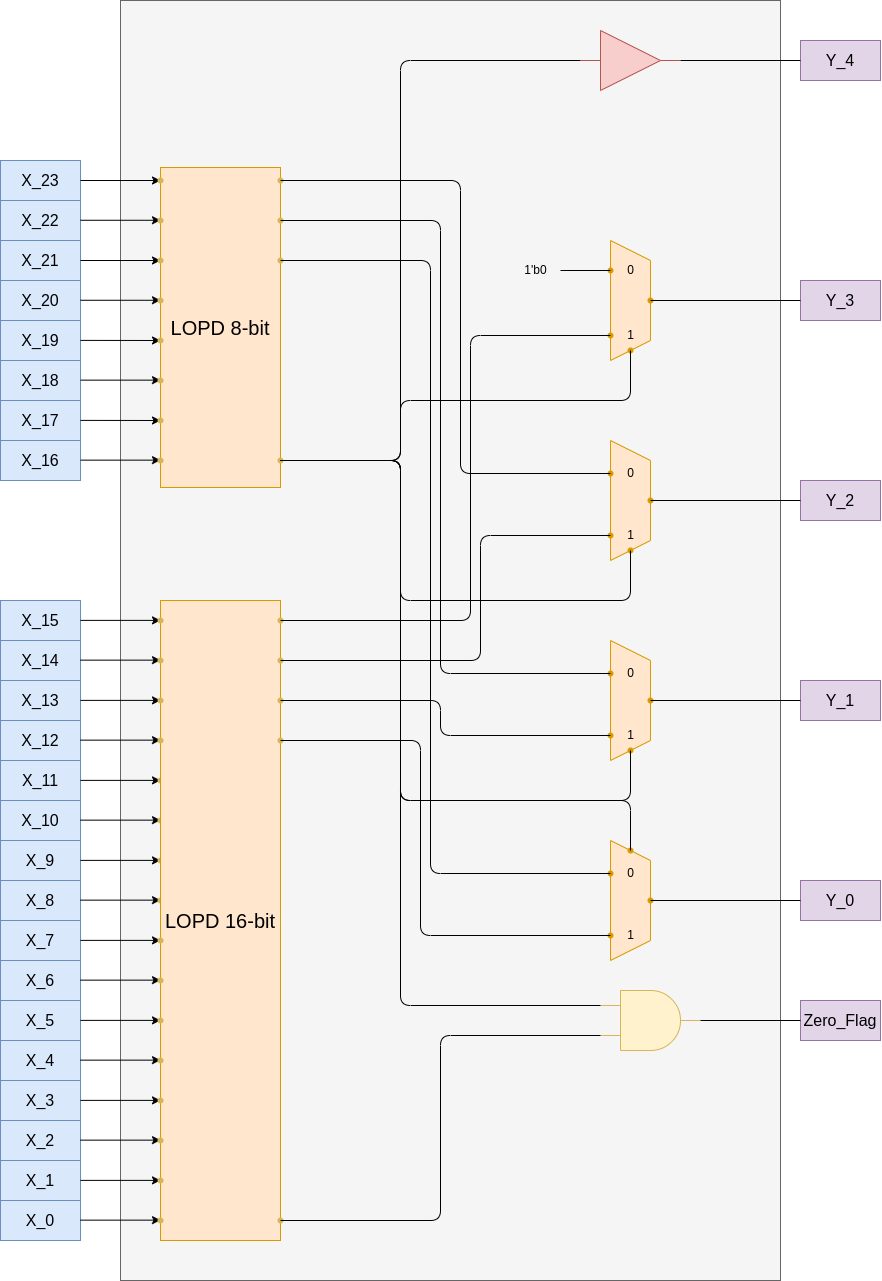
\includegraphics[width=.8\linewidth]{/home/noname/Documents/project_tiny/Ex3/20_doc/my-chapters/my-diagrams/Question2/LOPD_24bit.png}
	\caption{Sơ đồ logic của bộ LOPD 24-bit.}
\end{figure}

\answer{b}{Viết chương trình HDL mô tả mạch đã cho.}

\lstinputlisting[style=StyleCode, language=SystemVerilog, caption={Chương trình mô tả LOPD 4-bit.}]{/home/noname/Documents/project_tiny/Ex3/02_rtl/Question2/LOPD_4bit.sv}

\lstinputlisting[style=StyleCode, language=SystemVerilog, caption={Chương trình mô tả LOPD 8-bit.}]{/home/noname/Documents/project_tiny/Ex3/02_rtl/Question2/LOPD_8bit.sv}

\lstinputlisting[style=StyleCode, language=SystemVerilog, caption={Chương trình mô tả LOPD 16-bit.}]{/home/noname/Documents/project_tiny/Ex3/02_rtl/Question2/LOPD_16bit.sv}

\lstinputlisting[style=StyleCode, language=SystemVerilog, caption={Chương trình mô tả LOPD 24-bit.}]{/home/noname/Documents/project_tiny/Ex3/02_rtl/Question2/Question2.sv}

\answer{c}{Viết testbench cho mạch, thực hiện testbench với 100 mẫu và tính scoreboard của 100 mẫu đó.}

Đầu tiên nhóm em thưc hiện triển khai chứng minh kết quả đúng bằng giải thuật sau:

\begin{lstlisting}[style=StyleCode, language=SystemVerilog, caption={Giải thuật chứng minh kết quả của bộ LOPD 24-bit.}]
	function automatic logic [SIZE_LOP-1:0] Test_LOPD(
		input logic [SIZE_DATA-1:0]     f_i_data
	);
		logic [SIZE_DATA-1:0] t_temp;
		int cnt_position_1;
		begin
			t_temp = f_i_data;
			cnt_position_1 = 0;
			
			if(t_temp == 0) begin
				Test_LOPD = 0;
			end else begin
				while (t_temp[SIZE_DATA-1] == 0) begin
					t_temp = t_temp << 1;
					cnt_position_1 ++;
				end
				Test_LOPD = SIZE_DATA - cnt_position_1 - 1;
			end
		end
	endfunction
\end{lstlisting}


\question{Câu 3}

Thiết kế mạch tính tổng của 2 số 32-bit sử dụng giải thuật CLA (Carry Look-Ahead Adder) trong lý thuyết. Lưu ý: tách thành các bộ cộng 4-bit CLA.

Cho các standard cell là: cổng not, các cổng logic 2, 3, 4 ngõ vào.

\answer{a}{Thiết kế mạch theo phương pháp đã cho và chỉ được dùng các standard cell trên.}

Theo lý thuyết, ta định nghĩa được 2 tín hiệu quan trọng là:

\begin{itemize}[label=-]
	\item \textbf{Generate ($\mathbf{G_{i}}$)}: Sinh carry ngay tại bit đó: $G_{i} = A_{i} \& B_{i}$.
	\item \textbf{Propagate ($\mathbf{P_{i}}$)}: Cho phép carry từ bit trước đi qua: $P_{i} = A_{i} \oplus B_{i}$.
\end{itemize}

Dựa vào đó, ta thiết kế PG Generator (Propagate–Generate Generator) như sau:

\begin{figure}[H]
	\centering
	\includegraphics[width=.4\linewidth]{./my-chapters/my-images/Question3/hình 1.png}
	\caption{Sơ đồ logic của PG Generator.}
\end{figure}

Các tín hiệu $G_{i}$ và $P_{i}$ chính là đầu vào cho \textbf{Carry Generator} ở cấp kế tiếp. Biểu thức cho carry kế tiếp: $C_{i+1} = G_{i} | (P_{i} \& C_{in})$. Nếu thực hiện thế vào liên tục, ta được biểu thức như sau:
\[ C_1=G_0 | (P_0 \& C_{in}) \rightarrow C_2=G_2 | (G_0 \& P_1) | (P_1 \& P_2 \& C_{in}) \dots\]

Tức là \textit{tất cả các carry có thể tính song song} bằng các phép logic, không cần đợi ripple từng bit. Từ đó ta có thiết kế Carry Generator như sau:

\begin{figure}[H]
	\centering
	\includegraphics[width=.4\linewidth]{./my-chapters/my-images/Question3/hình 2.png}
	\caption{Sơ đồ logic của Carry Generator.}
\end{figure}

Sau khi biết các biết carry, ta tính tổng: $S_i = P_i \oplus C_{in}$. Từ đó, ta thiết kế bộ cộng CLA 4-bit như sau:

\begin{figure}[H]
	\centering
	\includegraphics[width=.7\linewidth]{./my-chapters/my-images/Question3/hình 3.png}
	\caption{Sơ đồ logic của bộ cộng 4-bit CLA.}
\end{figure}

Ngoài ra, cũng là sơ đồ logic ấy, ta có thể biểu diễn thiết kế khác như hình bên dưới:

\begin{figure}[H]
	\centering
	\includegraphics[width=.9\linewidth]{./my-chapters/my-images/Question3/hình 4.png}
	\caption{Block diagram của bộ cộng 4-bit CLA.}
\end{figure}

Từ những bộ trên, ta có được bộ tính tổng 2 số 32-bit bằng bộ cộng theo phương pháp CLA.

\begin{figure}[H]
	\centering
	\includegraphics[width=\linewidth]{./my-chapters/my-images/Question3/hình 5.png}
	\caption{Block diagram của bộ cộng 32-bit CLA.}
\end{figure}

\answer{b}{Viết chương trình HDL mô tả mạch đã cho.}

\lstinputlisting[style=StyleCode, language=SystemVerilog, caption={Chương trình mô tả CLA 4-bit.}]{./../02_rtl/Question3/cla_4bit.sv}

\lstinputlisting[style=StyleCode, language=SystemVerilog, caption={Chương trình mô tả CLA 32-bit.}]{./../02_rtl/Question3/cla_32bit.sv}

\answer{c}{Viết testbench cho mạch. Testbench thực hiện rải 100 mẫu và tính scoreboard của 100 mẫu đó.}

Nhóm em sử dụng dụng dấu \textsf{+} làm golden model để thực hiện kiểm tra kết quả test như sau:

\begin{lstlisting}[style=StyleCode, language=SystemVerilog, caption={Giải thuật chứng minh kết quả của bộ cộng CLA 32-bit.}]
	expected = {1'b0, tv_a} + {1'b0, tv_b} + tv_cin;
\end{lstlisting}

\begin{itemize}[label=-]
	\item Thực hiện kiểm thử (self-checking) với 100 mẫu random để áp vào DUT. So sánh với expected để cập nhật scoreboard.
	
	\begin{lstlisting}[style=StyleCode, language=SystemVerilog, caption={Sinh 100 mẫu random và thực hiện kiểm tra.}]
		$display("=== Start run_test (100 samples) ===");
		for (idx = 0; idx < 100; idx++) begin
			// --- generate testcase ---
			tv_a   = $urandom();
			tv_b   = $urandom();
			tv_cin = $urandom_range(0,1);
			A_tb   = tv_a;
			B_tb   = tv_b;
			Cin_tb = tv_cin;
			@(posedge clk);
			@(posedge clk);
			#1;
			// --- compute expected ---
			expected = {1'b0, tv_a} + {1'b0, tv_b} + tv_cin;
			got      = {Cout_tb, Sum_tb};
			// --- compare and display ---
			if (got == expected) begin
				pass_count++;
				$display("PASS [%0d] A=0x%08h B=0x%08h Cin=%0d => {Cout,Sum}=0x%09h",
					idx, tv_a, tv_b, tv_cin, got);
			end else begin
				fail_count++;
				$display("FAIL [%0d] A=0x%08h B=0x%08h Cin=%0d => got=0x%09h (exp=0x%09h)",
					idx, tv_a, tv_b, tv_cin, got, expected);
			end
		end
	\end{lstlisting}
	
	Kết quả
	
	\begin{lstlisting}[style=StyleResult, language=Result, caption={Kết quả test từng mẫu.}]
		# === Start run_test (100 samples) ===
		# PASS [0] A=0x2e45b278 B=0xd7aeae53 Cin=1 => {Cout,Sum}=0x105f460cc
		# PASS [1] A=0x1e3a4d4a B=0x4ba544f7 Cin=1 => {Cout,Sum}=0x069df9242
		# PASS [2] A=0xf331e3ec B=0x55820c15 Cin=0 => {Cout,Sum}=0x148b3f001
		# PASS [3] A=0xfb325326 B=0x4cd94c49 Cin=0 => {Cout,Sum}=0x1480b9f6f
		...
		# PASS [97] A=0xb68bc493 B=0x18b2dfcc Cin=0 => {Cout,Sum}=0x0cf3ea45f
		# PASS [98] A=0x3662a0de B=0x9cc1dc3f Cin=0 => {Cout,Sum}=0x0d3247d1d
		# PASS [99] A=0xafde0bca B=0xcf523f4e Cin=1 => {Cout,Sum}=0x17f304b19
	\end{lstlisting}
	
	\item Kết quả tổng kết.
	
	\begin{lstlisting}[style=StyleResult, language=SystemVerilog, caption={Kết quả của tổng kết của bài test.}]
		# === Test summary ===
		# Total samples = 100
		# PASS = 100
		# FAIL = 0
		# === End run_test ===
	\end{lstlisting}
\end{itemize}

\question{Câu 5}

Thiết kế một ALU thực hiện theo tính toán như bảng sau. Trong đó, $A$ và $B$ là 2 ngõ vào 8-bit. Các tín hiệu lựa chọn $S_{1}$, $S_{0}$ và $C_{in}$.

\begin{table}[H]
	\centering
	\caption{Bảng tính toán để thiết kế ALU.}
	\renewcommand{\arraystretch}{1.3}
	\setlength{\tabcolsep}{10pt}
	\begin{tabular}{|>{\centering\arraybackslash}m{1.5cm}
			|>{\centering\arraybackslash}m{5cm}
			|>{\centering\arraybackslash}m{5cm}|}
		\hline
		\textbf{S1S0} & \textbf{Cin = 0} & \textbf{Cin = 1} \\ \hline
		00 & $F = A + B$ (add) & $F = A + B + 1$ \\ \hline
		01 & $F = A$ (transfer) & $F = A + 1$ (increment) \\ \hline
		10 & $F = \bar{B}$ (complement) & $F = \bar{B} + 1$ (negate) \\ \hline
		11 & $F = A + \bar{B}$ & $F = A + \bar{B} + 1$ (subtract) \\ \hline
	\end{tabular}
	\label{tab: de_cau_5}
\end{table}

Cho các standard cell là: cổng not, các cổng logic 2 ngõ vào, mux 2-1, mux 4-1.


\answer{a}{Thiết kế mạch chỉ sử dụng các standard cell trên và chỉ được thiết kế 1 bộ cộng.}

Trước tiên, dựa vào Bảng \ref{tab: de_cau_5}, ta có thể rút ra được công thức tổng quát như sau: 
\[ F = A + B + C_{in} \]
Mà $C_{in}$ sẽ được điều khiển trực tiếp để đưa vào bộ cộng nên không cần dùng mux. Tóm lại ta chỉ cần quan tâm đến 2 toán hạng còn lại gọi là Op1 và Op2.

Ngoài ra, quan sát thấy tại $S_{1}S_{0} = 10$ chỉ có 1 toán hạng là $\bar{B}$ $\rightarrow$ Dùng mux 2-1 để chọn ra trường hợp đặc biệt này, dưới đây là hình ảnh thiết kế.

\begin{figure}[H]
	\centering
	\includegraphics[width=.9\linewidth]{./my-chapters/my-images/Question5/hình 6.png}
	\caption{Mux 2-1 cho toán hạng thứ nhất Op1.}
	\label{fig: 1}
\end{figure}

Hình \ref{fig: 1} là thiết kế được tóm gọn lại. Thực chất, vì là $A$ và $B$ là số 8-bit nên sẽ là 8 bộ mux 2-1 cho mỗi một bit.

Sau khi có toán hạng thứ nhất, ta tiến đến toán hạng thứ hai dựa vào toán hạng thứ nhất như sau:

\begin{table}[H]
	\centering
	\begin{tabular}{|>{\centering\arraybackslash}m{1.5cm}
			|>{\centering\arraybackslash}m{5cm}
			|>{\centering\arraybackslash}m{5cm}|}
		\hline
		\textbf{S1S0} & \textbf{Toán hạng 1 (Op1)} & \textbf{Toán hạng 2 (Op2)} \\ \hline
		00 & $A$ & $B$ \\ \hline
		01 & $A$ & $0$ \\ \hline
		10 & $\bar{B}$ & $0$ \\ \hline
		11 & $A$ & $\bar{B}$ \\ \hline
	\end{tabular}
	\caption{Bảng lựa chọn toán hạng thứ hai.}
	\label{tab: 2}
\end{table}

Dựa vào bảng \ref{tab: 2}, nhóm em chọn mux 4-1 để thiết kế cho phù hợp với 4 trường hợp trên. Tương tự, vì là thiết kế cho mỗi bit nên thực chất sẽ có đến 8 bộ mux 4-1.


\begin{figure}[H]
	\centering
	\includegraphics[width=.7\linewidth]{./my-chapters/my-images/Question5/hình 7.png}
	\caption{Mux 4-1 cho toán hạng thứ Op2.}
\end{figure}

Sau khi đã có đầy đủ hai toán hạng, việc còn lại là thiết kế bộ cộng với đầu vào là toán hạng thứ nhất và thứ hai đã chọn cùng với $C_{in}$. Tổng quát, bộ ALU sẽ có thiết kế như sau:

\begin{figure}[H]
	\centering
	\includegraphics[width=.9\linewidth]{./my-chapters/my-images/Question5/hình 8.png}
	\caption{Sơ đồ logic của bộ ALU.}
\end{figure}

Đối với bộ cộng, nhóm em sử dụng bộ cộng CLA 8-bit. Trước hết, cần phải xây dựng một khối CLA 4-bit như sau.


\begin{figure}[H]
	\centering
	\includegraphics[width=.9\linewidth]{./my-chapters/my-images/Question5/hình 9.png}
	\caption{4-bit Carry Lookahead Adder.}
\end{figure}

Dựa vào thiết kế này, ta nối 2 khối CLA 4-bit thành bộ cộng CLA 8-bit, cụ thể như hình dưới:

\begin{figure}[H]
	\centering
	\includegraphics[width=.9\linewidth]{./my-chapters/my-images/Question5/hình 10.png}
	\caption{8-bit Carry Lookahead Adder.}
\end{figure}

\answer{b}{Viết chương trình HDL mô tả mạch đã cho và viết testbench cho mạch}

\lstinputlisting[style=StyleCode, language=SystemVerilog, caption={Chương trình mô tả CLA 4-bit.}]{./../02_rtl/Question5/cla_4bit.sv}

\lstinputlisting[style=StyleCode, language=SystemVerilog, caption={Chương trình mô tả CLA 8-bit.}]{./../02_rtl/Question5/cla_8bit.sv}

\lstinputlisting[style=StyleCode, language=SystemVerilog, caption={Chương trình mô tả bộ ALU 8-bit.}]{./../02_rtl/Question5/alu_8bit.sv}

\answer{c}{Viết testbench cho mạch.}

Mục tiêu: Xác minh chức năng ALU 8-bit theo bảng $S_{1}$, $S_{0}$, $C_{in}$; đảm bảo $F$ và $C_{out}$ của DUT khớp với mô hình tham chiếu trên tập mẫu Directed + Random (100 mẫu tổng).

Ở đây, phương pháp nhóm em áp dụng là Functional Verification - Self-checking testbench. Cụ thể hơn, đây là Direct + Random Testing kết hợp Reference Model Comparison.

Nhóm sử dụng Reference Model để tính toán giá trị expected . Sau đó, thực hiện task để so sánh với giá trị expected và thực hiện cập nhật \textsf{PASS}/\textsf{FAIL}. Nhóm thực hiện test 100 trường hợp với những trường hợp và phương pháp test khác nhau.

\begin{itemize}[label=-]
	\item TestCase0: Thực hiện Directed Test kiểm tra trường hợp đầu vào đặc biệt mà logic dễ sai như sau:
	
	\begin{table}[H]
		\centering
		\begin{tabular}{|>{\centering\arraybackslash}m{1cm}
				|>{\centering\arraybackslash}m{3.5cm}
				|>{\arraybackslash}m{8.5cm}|}
			\hline
			\textbf{TH} & \textbf{Giá trị test A và B} & \textbf{Tác dụng test} \\ \hline
			1 & $A = 8'h00$, $B = 8'h00$ & Kiểm tra tính cộng cơ bản $(0 + 0 = 0)$ và xác nhận không có bit rác hoặc lỗi \textit{sign extension}. \\ \hline
			2 & $A = 8'hFF$, $B = 8'hFF$ & Kiểm tra tràn (\textit{overflow/carry}); khi $A = B = FF_h$, phép cộng cho $FE_h$ và \textit{carry} = 1. \\ \hline
			3 & $A = 8'hFF$, $B = 8'h01$ & Kiểm tra sinh \textit{Cout} khi cộng giá trị lớn nhất với 1 và xác nhận mạch \textit{carry propagate} hoạt động đúng ở bit thấp. \\ \hline
			4 & $A = 8'h80$, $B = 8'h80$ & Kiểm tra xử lý bit 7 (MSB), vì $0x80 = 1000\_0000$. Với signed, đây là vùng âm; với unsigned, kiểm tra tràn. \\ \hline
			5 & $A = 8'hAA$, $B = 8'h55$ & Kiểm tra truyền \textit{carry} xen kẽ. Các bit 1–0 xen kẽ giúp phát hiện lỗi nối bit hoặc XOR sai. \\ \hline
			6 & $A = 8'h55$, $B = 8'hAA$ & Kiểm tra tính đối xứng của phép cộng ($A + B = B + A$). \\ \hline
			7 & $A = 8'h0F$, $B = 8'hF0$ & Kiểm tra truyền \textit{carry} giữa nibble thấp–cao, đánh giá hoạt động cộng giữa các bit chéo. \\ \hline
		\end{tabular}
		\caption{Trường hợp đặc biệt được kiểm tra bằng Directed Test.}
	\end{table}
	
	\begin{lstlisting}[style=StyleCode, language=SystemVerilog, caption={Thực hiện Directed Test.}]
		task automatic run_test();
		logic [7:0] edgeA [0:6];
		logic [7:0] edgeB [0:6];
		int idx;
		int s1, s0, c;
		int rctl;
		begin
			total_tests = 0;
			errors = 0;
			test_count = 0;
			test_pass = 0;
			
			// --- Directed edge cases ---
			edgeA[0] = 8'h00; edgeB[0] = 8'h00;
			edgeA[1] = 8'hFF; edgeB[1] = 8'hFF;
			edgeA[2] = 8'hFF; edgeB[2] = 8'h01;
			edgeA[3] = 8'h80; edgeB[3] = 8'h80;
			edgeA[4] = 8'hAA; edgeB[4] = 8'h55;
			edgeA[5] = 8'h55; edgeB[5] = 8'hAA;
			edgeA[6] = 8'h0F; edgeB[6] = 8'hF0;
			
			$display("\n========== STARTING DIRECTED TESTS ==========\n");
			for (idx = 0; idx <= 6; idx++) begin
				for (s1 = 0; s1 < 2; s1++) begin
					for (s0 = 0; s0 < 2; s0++) begin
						for (c = 0; c < 2; c++) begin
							apply_and_check(edgeA[idx], edgeB[idx], s1, s0, c, "Direct");
						end
					end
				end
			end
		end
		endtask
	\end{lstlisting}
	
	Kết quả 
	
	\begin{lstlisting}[style=StyleResult, language=Result, caption={Kết quả mô phỏng Directed Test.}]
		# ========== STARTING DIRECTED TESTS ==========
		# 
		# [TIME:   1000] [Direct] A=00 B=00 S1S0=00 Cin=0 | F=00 Cout=0
		# => PASS: Expect: 00 (0), DUT: 00 (0)
		# ------------------------------------------------------------
		# [TIME:   2000] [Direct] A=00 B=00 S1S0=00 Cin=1 | F=01 Cout=0
		# => PASS: Expect: 01 (1), DUT: 01 (1)
		# ------------------------------------------------------------
		# [TIME:   3000] [Direct] A=00 B=00 S1S0=01 Cin=0 | F=00 Cout=0
		# => PASS: Expect: 00 (0), DUT: 00 (0)
		# ------------------------------------------------------------
		# [TIME:   4000] [Direct] A=00 B=00 S1S0=01 Cin=1 | F=01 Cout=0
		# => PASS: Expect: 01 (1), DUT: 01 (1)
		# ------------------------------------------------------------
		# [TIME:   5000] [Direct] A=00 B=00 S1S0=10 Cin=0 | F=ff Cout=0
		# => PASS: Expect: ff (255), DUT: ff (255)
		# ------------------------------------------------------------
		# [TIME:   6000] [Direct] A=00 B=00 S1S0=10 Cin=1 | F=00 Cout=1
		# => PASS: Expect: 00 (0), DUT: 00 (0)
		# ------------------------------------------------------------
		# [TIME:   7000] [Direct] A=00 B=00 S1S0=11 Cin=0 | F=ff Cout=0
		# => PASS: Expect: ff (255), DUT: ff (255)
		# ------------------------------------------------------------
		# [TIME:   8000] [Direct] A=00 B=00 S1S0=11 Cin=1 | F=00 Cout=1
		# => PASS: Expect: 00 (0), DUT: 00 (0)
		# ------------------------------------------------------------
		# [TIME:   9000] [Direct] A=ff B=ff S1S0=00 Cin=0 | F=fe Cout=1
		# => PASS: Expect: fe (254), DUT: fe (254)
		# ------------------------------------------------------------
		# [TIME:  10000] [Direct] A=ff B=ff S1S0=00 Cin=1 | F=ff Cout=1
		# => PASS: Expect: ff (255), DUT: ff (255)
		# ------------------------------------------------------------
		# [TIME:  11000] [Direct] A=ff B=ff S1S0=01 Cin=0 | F=ff Cout=0
		# => PASS: Expect: ff (255), DUT: ff (255)
		# ------------------------------------------------------------
		# [TIME:  12000] [Direct] A=ff B=ff S1S0=01 Cin=1 | F=00 Cout=1
		# => PASS: Expect: 00 (0), DUT: 00 (0)
		# ------------------------------------------------------------
		# [TIME:  13000] [Direct] A=ff B=ff S1S0=10 Cin=0 | F=00 Cout=0
		# => PASS: Expect: 00 (0), DUT: 00 (0)
		# ------------------------------------------------------------
		# [TIME:  14000] [Direct] A=ff B=ff S1S0=10 Cin=1 | F=01 Cout=0
		# => PASS: Expect: 01 (1), DUT: 01 (1)
		# ------------------------------------------------------------
		# [TIME:  15000] [Direct] A=ff B=ff S1S0=11 Cin=0 | F=ff Cout=0
		# => PASS: Expect: ff (255), DUT: ff (255)
		# ------------------------------------------------------------
		# [TIME:  16000] [Direct] A=ff B=ff S1S0=11 Cin=1 | F=00 Cout=1
		# => PASS: Expect: 00 (0), DUT: 00 (0)
		# ------------------------------------------------------------
		# [TIME:  17000] [Direct] A=ff B=01 S1S0=00 Cin=0 | F=00 Cout=1
		# => PASS: Expect: 00 (0), DUT: 00 (0)
		# ------------------------------------------------------------
		# [TIME:  18000] [Direct] A=ff B=01 S1S0=00 Cin=1 | F=01 Cout=1
		# => PASS: Expect: 01 (1), DUT: 01 (1)
		# ------------------------------------------------------------
		# [TIME:  19000] [Direct] A=ff B=01 S1S0=01 Cin=0 | F=ff Cout=0
		# => PASS: Expect: ff (255), DUT: ff (255)
		# ------------------------------------------------------------
		# [TIME:  20000] [Direct] A=ff B=01 S1S0=01 Cin=1 | F=00 Cout=1
		# => PASS: Expect: 00 (0), DUT: 00 (0)
		# ------------------------------------------------------------
		# [TIME:  21000] [Direct] A=ff B=01 S1S0=10 Cin=0 | F=fe Cout=0
		# => PASS: Expect: fe (254), DUT: fe (254)
		# ------------------------------------------------------------
		# [TIME:  22000] [Direct] A=ff B=01 S1S0=10 Cin=1 | F=ff Cout=0
		# => PASS: Expect: ff (255), DUT: ff (255)
		# ------------------------------------------------------------
		# [TIME:  23000] [Direct] A=ff B=01 S1S0=11 Cin=0 | F=fd Cout=1
		# => PASS: Expect: fd (253), DUT: fd (253)
		# ------------------------------------------------------------
		# [TIME:  24000] [Direct] A=ff B=01 S1S0=11 Cin=1 | F=fe Cout=1
		# => PASS: Expect: fe (254), DUT: fe (254)
		# ------------------------------------------------------------
		# [TIME:  25000] [Direct] A=80 B=80 S1S0=00 Cin=0 | F=00 Cout=1
		# => PASS: Expect: 00 (0), DUT: 00 (0)
		# ------------------------------------------------------------
		# [TIME:  26000] [Direct] A=80 B=80 S1S0=00 Cin=1 | F=01 Cout=1
		# => PASS: Expect: 01 (1), DUT: 01 (1)
		# ------------------------------------------------------------
		# [TIME:  27000] [Direct] A=80 B=80 S1S0=01 Cin=0 | F=80 Cout=0
		# => PASS: Expect: 80 (128), DUT: 80 (128)
		# ------------------------------------------------------------
		# [TIME:  28000] [Direct] A=80 B=80 S1S0=01 Cin=1 | F=81 Cout=0
		# => PASS: Expect: 81 (129), DUT: 81 (129)
		# ------------------------------------------------------------
		# [TIME:  29000] [Direct] A=80 B=80 S1S0=10 Cin=0 | F=7f Cout=0
		# => PASS: Expect: 7f (127), DUT: 7f (127)
		# ------------------------------------------------------------
		# [TIME:  30000] [Direct] A=80 B=80 S1S0=10 Cin=1 | F=80 Cout=0
		# => PASS: Expect: 80 (128), DUT: 80 (128)
		# ------------------------------------------------------------
		# [TIME:  31000] [Direct] A=80 B=80 S1S0=11 Cin=0 | F=ff Cout=0
		# => PASS: Expect: ff (255), DUT: ff (255)
		# ------------------------------------------------------------
		# [TIME:  32000] [Direct] A=80 B=80 S1S0=11 Cin=1 | F=00 Cout=1
		# => PASS: Expect: 00 (0), DUT: 00 (0)
		# ------------------------------------------------------------
		# [TIME:  33000] [Direct] A=aa B=55 S1S0=00 Cin=0 | F=ff Cout=0
		# => PASS: Expect: ff (255), DUT: ff (255)
		# ------------------------------------------------------------
		# [TIME:  34000] [Direct] A=aa B=55 S1S0=00 Cin=1 | F=00 Cout=1
		# => PASS: Expect: 00 (0), DUT: 00 (0)
		# ------------------------------------------------------------
		# [TIME:  35000] [Direct] A=aa B=55 S1S0=01 Cin=0 | F=aa Cout=0
		# => PASS: Expect: aa (170), DUT: aa (170)
		# ------------------------------------------------------------
		# [TIME:  36000] [Direct] A=aa B=55 S1S0=01 Cin=1 | F=ab Cout=0
		# => PASS: Expect: ab (171), DUT: ab (171)
		# ------------------------------------------------------------
		# [TIME:  37000] [Direct] A=aa B=55 S1S0=10 Cin=0 | F=aa Cout=0
		# => PASS: Expect: aa (170), DUT: aa (170)
		# ------------------------------------------------------------
		# [TIME:  38000] [Direct] A=aa B=55 S1S0=10 Cin=1 | F=ab Cout=0
		# => PASS: Expect: ab (171), DUT: ab (171)
		# ------------------------------------------------------------
		# [TIME:  39000] [Direct] A=aa B=55 S1S0=11 Cin=0 | F=54 Cout=1
		# => PASS: Expect: 54 (84), DUT: 54 (84)
		# ------------------------------------------------------------
		# [TIME:  40000] [Direct] A=aa B=55 S1S0=11 Cin=1 | F=55 Cout=1
		# => PASS: Expect: 55 (85), DUT: 55 (85)
		# ------------------------------------------------------------
		# [TIME:  41000] [Direct] A=55 B=aa S1S0=00 Cin=0 | F=ff Cout=0
		# => PASS: Expect: ff (255), DUT: ff (255)
		# ------------------------------------------------------------
		# [TIME:  42000] [Direct] A=55 B=aa S1S0=00 Cin=1 | F=00 Cout=1
		# => PASS: Expect: 00 (0), DUT: 00 (0)
		# ------------------------------------------------------------
		# [TIME:  43000] [Direct] A=55 B=aa S1S0=01 Cin=0 | F=55 Cout=0
		# => PASS: Expect: 55 (85), DUT: 55 (85)
		# ------------------------------------------------------------
		# [TIME:  44000] [Direct] A=55 B=aa S1S0=01 Cin=1 | F=56 Cout=0
		# => PASS: Expect: 56 (86), DUT: 56 (86)
		# ------------------------------------------------------------
		# [TIME:  45000] [Direct] A=55 B=aa S1S0=10 Cin=0 | F=55 Cout=0
		# => PASS: Expect: 55 (85), DUT: 55 (85)
		# ------------------------------------------------------------
		# [TIME:  46000] [Direct] A=55 B=aa S1S0=10 Cin=1 | F=56 Cout=0
		# => PASS: Expect: 56 (86), DUT: 56 (86)
		# ------------------------------------------------------------
		# [TIME:  47000] [Direct] A=55 B=aa S1S0=11 Cin=0 | F=aa Cout=0
		# => PASS: Expect: aa (170), DUT: aa (170)
		# ------------------------------------------------------------
		# [TIME:  48000] [Direct] A=55 B=aa S1S0=11 Cin=1 | F=ab Cout=0
		# => PASS: Expect: ab (171), DUT: ab (171)
		# ------------------------------------------------------------
		# [TIME:  49000] [Direct] A=0f B=f0 S1S0=00 Cin=0 | F=ff Cout=0
		# => PASS: Expect: ff (255), DUT: ff (255)
		# ------------------------------------------------------------
		# [TIME:  50000] [Direct] A=0f B=f0 S1S0=00 Cin=1 | F=00 Cout=1
		# => PASS: Expect: 00 (0), DUT: 00 (0)
		# ------------------------------------------------------------
		# [TIME:  51000] [Direct] A=0f B=f0 S1S0=01 Cin=0 | F=0f Cout=0
		# => PASS: Expect: 0f (15), DUT: 0f (15)
		# ------------------------------------------------------------
		# [TIME:  52000] [Direct] A=0f B=f0 S1S0=01 Cin=1 | F=10 Cout=0
		# => PASS: Expect: 10 (16), DUT: 10 (16)
		# ------------------------------------------------------------
		# [TIME:  53000] [Direct] A=0f B=f0 S1S0=10 Cin=0 | F=0f Cout=0
		# => PASS: Expect: 0f (15), DUT: 0f (15)
		# ------------------------------------------------------------
		# [TIME:  54000] [Direct] A=0f B=f0 S1S0=10 Cin=1 | F=10 Cout=0
		# => PASS: Expect: 10 (16), DUT: 10 (16)
		# ------------------------------------------------------------
		# [TIME:  55000] [Direct] A=0f B=f0 S1S0=11 Cin=0 | F=1e Cout=0
		# => PASS: Expect: 1e (30), DUT: 1e (30)
		# ------------------------------------------------------------
		# [TIME:  56000] [Direct] A=0f B=f0 S1S0=11 Cin=1 | F=1f Cout=0
		# => PASS: Expect: 1f (31), DUT: 1f (31)
		# ------------------------------------------------------------
	\end{lstlisting}
	
	\item TestCase1: test trường hợp toàn zero. Để xác nhận là mô phỏng ổn, đảm bảo mạch không tạo nhiễu hay glitch.
	
	\begin{lstlisting}[style=StyleCode, language=SystemVerilog, caption={Thực hiện kiểm tra zero case.}]
		task automatic run_test();
		logic [7:0] edgeA [0:6];
		logic [7:0] edgeB [0:6];
		int idx;
		int s1, s0, c;
		int rctl;
		begin
			total_tests = 0;
			errors = 0;
			test_count = 0;
			test_pass = 0;
			$display("\n========== ZERO CASE TEST ==========\n");
			apply_and_check(8'h00, 8'h00, 0, 0, 0, "Zero");
		end
		endtask
	\end{lstlisting}
	
	Kết quả
	
	\begin{lstlisting}[style=StyleResult, language=Result, caption={Kết quả mô phỏng Directed Test.}]
		# ========== ZERO CASE TEST ==========
		# 
		# [TIME:  57000] [Zero] A=00 B=00 S1S0=00 Cin=0 | F=00 Cout=0
		# => PASS: Expect: 00 (0), DUT: 00 (0)
		# ------------------------------------------------------------
	\end{lstlisting}
	
	\item TestCase2: Random Test sau khi chạy Directed test và zero case trước đó: Sinh ngẫu nhiên giá trị $A$, $B$, $S_{1}$, $S_{0}$, $C_{in}$ bằng hàm \$urandom(seed). Dừng khi đạt 100 mẫu test tổng cộng.
	
	\begin{lstlisting}[style=StyleCode, language=SystemVerilog, caption={Thực hiện Random Test.}]
		task automatic run_test();
		logic [7:0] edgeA [0:6];
		logic [7:0] edgeB [0:6];
		int idx;
		int s1, s0, c;
		int rctl;
		begin
			total_tests = 0;
			errors = 0;
			test_count = 0;
			test_pass = 0;
			seed = 32'hCAFEBABE;
			while (total_tests < 100) begin
				A = $urandom(seed) & 8'hFF;
				B = $urandom(seed + 1) & 8'hFF;
				rctl = $urandom(seed + 2) % 8;
				S1 = (rctl >> 2) & 1;
				S0 = (rctl >> 1) & 1;
				Cin = rctl & 1;
				#1;
				apply_and_check(A, B, S1, S0, Cin, "Random");
				seed = seed + 12345;
			end
		end
		endtask
	\end{lstlisting}
	
	Kết quả 
	
	\begin{lstlisting}[style=StyleResult, language=Result, caption={Kết quả mô phỏng Directed Test.}]
		# ========== STARTING RANDOM TESTS ==========
		# 
		# [TIME:  59000] [Random] A=07 B=5b S1S0=11 Cin=1 | F=ac Cout=0
		# => PASS: Expect: ac (172), DUT: ac (172)
		# ------------------------------------------------------------
		# [TIME:  61000] [Random] A=46 B=63 S1S0=00 Cin=1 | F=aa Cout=0
		# => PASS: Expect: aa (170), DUT: aa (170)
		# ------------------------------------------------------------
		# [TIME:  63000] [Random] A=07 B=a0 S1S0=00 Cin=0 | F=a7 Cout=0
		# => PASS: Expect: a7 (167), DUT: a7 (167)
		...
		# [TIME: 141000] [Random] A=8a B=79 S1S0=11 Cin=1 | F=11 Cout=1
		# => PASS: Expect: 11 (17), DUT: 11 (17)
		# ------------------------------------------------------------
		# [TIME: 143000] [Random] A=1f B=93 S1S0=11 Cin=1 | F=8c Cout=0
		# => PASS: Expect: 8c (140), DUT: 8c (140)
		# ------------------------------------------------------------
	\end{lstlisting}
	
	\item Kết quả tổng kết.
	
	\begin{lstlisting}[style=StyleResult, language=SystemVerilog, caption={Kết quả của tổng kết của bài test.}]
		# ============================================
		# =============== TEST SUMMARY ===============
		# Total test cases : 100
		# Passed            : 100
		# Failed            : 0
		# Pass rate         : 100.00 %
		# ============================================
	\end{lstlisting}
\end{itemize}
%\question{Câu 6}

Thiết kế một bộ sắp xếp song song như hình dưới, mô tả giải thuật sắp xếp 8 mẫu ngõ vào $x_{1}$, $x_{2}$,$\dots, x_{8}$, và cho ngõ ra là $y_{1}$, $y_{2}$, $\dots, y_{8}$ theo thứ tự giảm dần (hoặc tăng dần).

\begin{figure}[H]
	\centering
	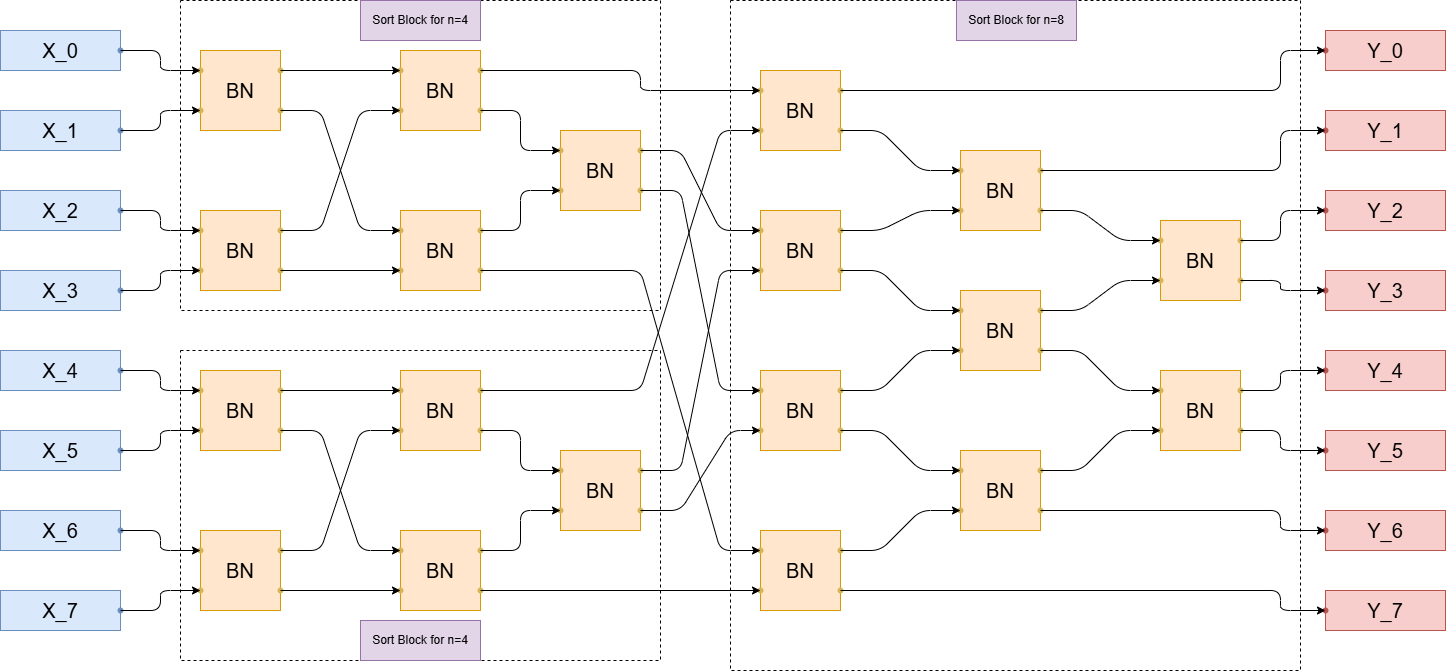
\includegraphics[width=\linewidth]{./my-chapters/my-diagrams/Question6/debai.png}
\end{figure}

Trong đó, mỗi bộ BN (Bitonic Sort) có cấu trúc như hình:

\begin{figure}[H]
	\centering
	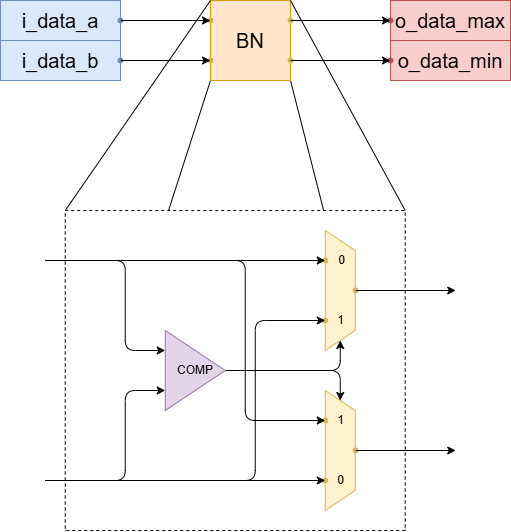
\includegraphics[width=.4z\linewidth]{./my-chapters/my-diagrams/Question6/Swap_and_compare.png}
\end{figure}

Cho các standard cell là: Cổng NOT, các cổng logic 2 ngõ vào, Mux 2-1, Mux 4-1.
\end{document}
